\section{A state-wise lower bound on the gap}
\label{sec:bound}

We now bound $\kappa - R$ from below for every state of the pendulum, using only exact identities, an elementary inequality for the strain, the bound~\eqref{eq:Hbound}, and a weighted Cram\'er--Rao inequality~\cite{rao1945,cramer1946} along the contracting direction. Let $\delta = X_q - \pi$ and
\begin{align}
\gamma(y) &= 1 - \bar a(y) = \E[\sin^2(\delta/2)\,|\,y] \in [0,1], \\
\omega(y) &= \sigma^2\,[H_{vv}(y)]_+ \in [0,1], \\
u(y) &= \sqrt2\,\left(\E[X_q\,|\,y] - \pi\right),
\end{align}
the local strain deficit, the focus weight across the stretching direction, and the signed offset of the posterior mean from the hyperbolic point, scaled by $\sqrt2$. Let $j = \E[\omega(Y)]$, $s_w$ the $w$ component of the score, and $[x]_\pm = \max(\pm x, 0)$. Define
\begin{equation}
\Theta' = \frac{|\E[\omega u s_w]|}{j}\sqrt{\frac{F_{ww}}{\E[\omega s_w^2]}},
\label{eq:Theta}
\end{equation}
\begin{align}
\tilde\varepsilon = \frac{1}{\tr F}\Bigl\{&\sigma^{-2}\,\E\!\left[\omega\left(\tfrac{1}{48}\E[\delta^4|Y] - \tfrac14\Var(X_q|Y)\right)\right] \nonumber\\
&+ \E\!\left[\gamma\,[H_{vv}]_-\right] + \E[\gamma H_{ww}]\Bigr\}.
\label{eq:epstilde}
\end{align}

\begin{theorem}[State-wise lower bound]
\label{thm:statewise}
For every state of the pendulum and every $\sigma > 0$,
\begin{equation}
1 - R \;\geq\; \frac{\Theta'\sigma}{1 + \Theta'\sigma/2} - \tilde\varepsilon - D ,
\label{eq:statewise}
\end{equation}
with $D$ the Stein defect of Proposition~\ref{prop:decomposition}.
\end{theorem}

The proof is in Appendix~\ref{app:bound}. It uses four inequalities: $\sin^2(x/2) \geq x^2/4 - x^4/48$; the Cauchy--Schwarz inequality with weight $\omega$, $\E[\omega u^2]\,\E[\omega s_w^2] \geq \E[\omega u s_w]^2$, which reduces for $\omega \equiv 1$ to the Cram\'er--Rao inequality along $w$; the bound $H \preceq \sigma^{-2}I$; and an elementary minimization. No sign condition is needed.

The quantity $\Theta'$ measures how the focus across the stretching direction is distributed along the contracting direction. For a zero-width segment exactly along $w$ the focus is uniform, $\omega \equiv 1$, and $\Theta' = 1 - \sigma^2 F_{ww} \to 1$. For the best Gaussian state, a slightly tilted segment, the bound nearly reproduces the gap: at $\sigma = 10^{-3}$ it is $0.9988\,\sigma$ against the exact $0.9991\,\sigma$. A fan concentrates its focus near the crossing point, and $\Theta'$ decreases. An immediate consequence is a uniform gap on any class of states on which $\Theta'$ is bounded below.

\begin{corollary}[Conditional uniform gap]
\label{cor:uniform}
If, on a class of states, $\Theta' \geq \Theta_0 > 0$ and $\tilde\varepsilon + D \leq \eta\sigma$, then every state of the class satisfies
\begin{equation}
1 - R \geq \left(\frac{\Theta_0}{1 + \Theta_0\sigma/2} - \eta\right)\sigma .
\end{equation}
For Gaussian states, no condition is needed: $1 - R \geq 1 - R^*(\sigma) = \sigma - \tfrac78\sigma^2 + \cdots$ by Theorem~\ref{thm:pendulum}.
\end{corollary}

\begin{figure*}[t]
\centering
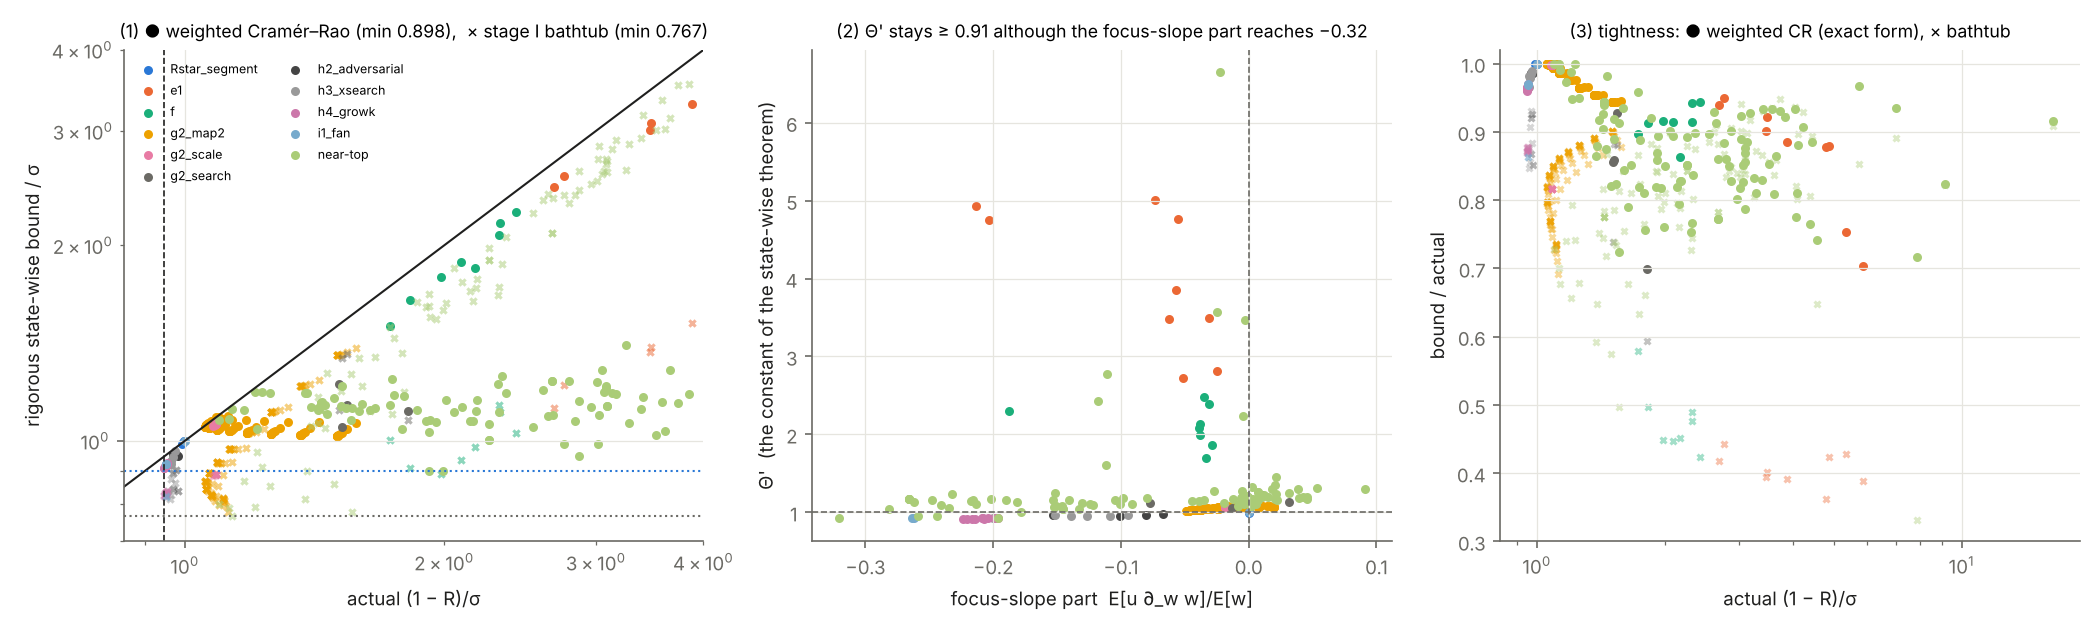
\includegraphics[width=0.95\textwidth]{figures/fig5_bound.png}
\caption{State-wise lower bound for the pendulum. (1) Bound of Theorem~\ref{thm:statewise} (dots) and the earlier, weaker bound that only uses $\omega \leq 1$ (crosses), against the actual gap, for all stored states with $\sigma \leq 10^{-2}$. (2) $\Theta'$ against the focus-slope part of $\E[\omega u s_w]/j$. (3) Ratio of bound to actual gap.}
\label{fig:bound}
\end{figure*}

\begin{observation}[Tightness]
\label{obs:bound}
On all $268$ stored pendulum states with $\sigma \leq 10^{-2}$, including the fans and adversarial states of Sec.~\ref{sec:mixtures}, $\Theta' \geq 0.9125$ and the bound~\eqref{eq:statewise} is at least $0.898\,\sigma$ (Fig.~\ref{fig:bound}). Before the minimization over the auxiliary variable it is at least $0.909\,\sigma$. The smallest actual gap among these states is $0.946\,\sigma$. For the $82$ states with gap below $1.1\,\sigma$ the bound is within $5\%$ of the actual gap.
\end{observation}

What prevents a uniform bound is the following. Integrating by parts along $w$,
\begin{equation}
-\E[\omega u s_w] = \E[\omega\,\partial_w u] + \E[u\,\partial_w\omega] .
\label{eq:ibp}
\end{equation}
The first, geometric term is close to $j$ (at least $0.963\,j$ on all stored states). The second, the \emph{focus slope}, is negative for fans, between $-0.2\,j$ and $-0.3\,j$; it is the mechanism by which mixtures beat the best Gaussian state. Bounding it requires control of $\partial_w H_{vv}$, a third derivative of $\ln\rho_C$, that is, of third posterior cumulants. The bound $H \preceq \sigma^{-2}I$ limits how sharp the focus can be but not how fast it can change, and for mixtures with crossing components the focus can change on short scales. A uniform bound also needs $\tilde\varepsilon + D = o(\sigma)$: $\tilde\varepsilon$ contains the valley term $\E[\gamma[H_{vv}]_-]$, which is not controlled in general, and $D$ can be positive. Numerically both are small near the hyperbolic point ($D/\sigma \leq 0.0022$ for $\sigma \leq 10^{-2}$). Replacing $\omega$ by a weight that is only allowed to vary slowly along $w$ removes the focus slope at the price of a smaller weight (Appendix~\ref{app:bound}, Proposition~\ref{prop:smooth}); under explicit conditions this gives a uniform gap, for example $0.344\,\sigma$ on the stored states concentrated near the hyperbolic point, but the conditions themselves are observed rather than proved.
